% Options for packages loaded elsewhere
\PassOptionsToPackage{unicode}{hyperref}
\PassOptionsToPackage{hyphens}{url}
%
\documentclass[
]{article}
\usepackage{amsmath,amssymb}
\usepackage{lmodern}
\usepackage{ifxetex,ifluatex}
\ifnum 0\ifxetex 1\fi\ifluatex 1\fi=0 % if pdftex
  \usepackage[T1]{fontenc}
  \usepackage[utf8]{inputenc}
  \usepackage{textcomp} % provide euro and other symbols
\else % if luatex or xetex
  \usepackage{unicode-math}
  \defaultfontfeatures{Scale=MatchLowercase}
  \defaultfontfeatures[\rmfamily]{Ligatures=TeX,Scale=1}
\fi
% Use upquote if available, for straight quotes in verbatim environments
\IfFileExists{upquote.sty}{\usepackage{upquote}}{}
\IfFileExists{microtype.sty}{% use microtype if available
  \usepackage[]{microtype}
  \UseMicrotypeSet[protrusion]{basicmath} % disable protrusion for tt fonts
}{}
\makeatletter
\@ifundefined{KOMAClassName}{% if non-KOMA class
  \IfFileExists{parskip.sty}{%
    \usepackage{parskip}
  }{% else
    \setlength{\parindent}{0pt}
    \setlength{\parskip}{6pt plus 2pt minus 1pt}}
}{% if KOMA class
  \KOMAoptions{parskip=half}}
\makeatother
\usepackage{xcolor}
\IfFileExists{xurl.sty}{\usepackage{xurl}}{} % add URL line breaks if available
\IfFileExists{bookmark.sty}{\usepackage{bookmark}}{\usepackage{hyperref}}
\hypersetup{
  pdftitle={Music Descriptors Supplementary Materials},
  pdfauthor={Brendon Mizener},
  hidelinks,
  pdfcreator={LaTeX via pandoc}}
\urlstyle{same} % disable monospaced font for URLs
\usepackage[margin=1in]{geometry}
\usepackage{graphicx}
\makeatletter
\def\maxwidth{\ifdim\Gin@nat@width>\linewidth\linewidth\else\Gin@nat@width\fi}
\def\maxheight{\ifdim\Gin@nat@height>\textheight\textheight\else\Gin@nat@height\fi}
\makeatother
% Scale images if necessary, so that they will not overflow the page
% margins by default, and it is still possible to overwrite the defaults
% using explicit options in \includegraphics[width, height, ...]{}
\setkeys{Gin}{width=\maxwidth,height=\maxheight,keepaspectratio}
% Set default figure placement to htbp
\makeatletter
\def\fps@figure{htbp}
\makeatother
\setlength{\emergencystretch}{3em} % prevent overfull lines
\providecommand{\tightlist}{%
  \setlength{\itemsep}{0pt}\setlength{\parskip}{0pt}}
\setcounter{secnumdepth}{-\maxdimen} % remove section numbering
% Manuscript styling
\usepackage{upgreek}
\usepackage{caption}

\captionsetup{font=singlespacing,justification=justified}

% Table formatting
\usepackage{longtable}
\usepackage{lscape}
% \usepackage[counterclockwise]{rotating}   % Landscape page setup for large tables
\usepackage{multirow}		% Table styling
\usepackage{tabularx}		% Control Column width
\usepackage[flushleft]{threeparttable}	% Allows for three part tables with a specified notes section
\usepackage{threeparttablex}            % Lets threeparttable work with longtable
\usepackage{endfloat}

% Create new environments so endfloat can handle them
% \newenvironment{ltable}
%   {\begin{landscape}\begin{center}\begin{threeparttable}}
%   {\end{threeparttable}\end{center}\end{landscape}}
\newenvironment{lltable}{\begin{landscape}\begin{center}\begin{ThreePartTable}}{\end{ThreePartTable}\end{center}\end{landscape}}

% Enables adjusting longtable caption width to table width
% Solution found at http://golatex.de/longtable-mit-caption-so-breit-wie-die-tabelle-t15767.html
\makeatletter
\newcommand\LastLTentrywidth{1em}
\newlength\longtablewidth
\setlength{\longtablewidth}{1in}
\newcommand{\getlongtablewidth}{\begingroup \ifcsname LT@\roman{LT@tables}\endcsname \global\longtablewidth=0pt \renewcommand{\LT@entry}[2]{\global\advance\longtablewidth by ##2\relax\gdef\LastLTentrywidth{##2}}\@nameuse{LT@\roman{LT@tables}} \fi \endgroup}

% \setlength{\parindent}{0.5in}
% \setlength{\parskip}{0pt plus 0pt minus 0pt}

% \usepackage{etoolbox}
\makeatletter
\patchcmd{\HyOrg@maketitle}
  {\section{\normalfont\normalsize\abstractname}}
  {\section*{\normalfont\normalsize\abstractname}}
  {}{\typeout{Failed to patch abstract.}}
\patchcmd{\HyOrg@maketitle}
  {\section{\protect\normalfont{\@title}}}
  {\section*{\protect\normalfont{\@title}}}
  {}{\typeout{Failed to patch title.}}
\makeatother

\usepackage{deluxetable}
\usepackage{graphicx}
\usepackage{subcaption}
\usepackage{rotating}
\usepackage{float}
\usepackage{booktabs}
\usepackage{longtable}
\usepackage{array}
\usepackage{multirow}
\usepackage{wrapfig}
\usepackage{float}
\usepackage{colortbl}
\usepackage{pdflscape}
\usepackage{tabu}
\usepackage{threeparttable}
\usepackage{threeparttablex}
\usepackage[normalem]{ulem}
\usepackage{makecell}
\usepackage{xcolor}
\ifluatex
  \usepackage{selnolig}  % disable illegal ligatures
\fi

\title{Music Descriptors Supplementary Materials}
\author{Brendon Mizener}
\date{5/12/2021}

\begin{document}
\maketitle

\hypertarget{supplementary-materials-experiment-1}{%
\section{Supplementary Materials: Experiment
1}\label{supplementary-materials-experiment-1}}

\begin{lltable}
\begin{footnotesize}
\begin{longtable}{p{0.2\textwidth}p{0.2\textwidth}p{0.2\textwidth}p{0.2\textwidth}p{0.2\textwidth}p{0.2\textwidth}}\noalign{\getlongtablewidth\global\LTcapwidth=\longtablewidth}
\caption{\label{tab:qualitiestable}Musical Qualities and the provided survey response options, English.}\\
\toprule[.8pt]
 \multicolumn{1}{c}{Harmonic Material} & \multicolumn{1}{c}{Tempo} & \multicolumn{1}{c}{Meter} & \multicolumn{1}{c}{Density} & \multicolumn{1}{c}{Genre} & \multicolumn{1}{c}{Articulation}\\
 \midrule
      Diatonic: Major & Very slow & Simple Duple & Very sparse & Baroque & Staccato \\
      Diatonic: Minor & Slow & Simple Triple & Moderately sparse & Classical & Marcato \\
      Blues & Moderately Slow & Simple Quadruple  & More sparse than dense & Romantic & Legato\\
      Chromatic & Moderate & Compound Duple & More dense than sparse & Impressionist & Tenuto\\
      Whole tone & Moderately Fast & Compound Triple & Moderately Dense & Modern & Other \\       
      Modal  & Fast & Compound Quadruple & Very Dense & Jazz/Blues & \\
      Quintal/Quartal  & Very Fast & Complex & & Contemporary & \\
      Ambiguous  & & & & Other & \\
      Other  & & & & & \\
\bottomrule\addlinespace[.5em]
 & \multicolumn{1}{c}{Contour} & \multicolumn{1}{c}{Motion} & \multicolumn{1}{c}{Range} & \multicolumn{1}{c}{Dynamics} & \\
 \cmidrule[.5pt]{2-5}
  & Ascending & Conjunct & Narrow & Soft & \\
  & Descending & Disjunct & Moderate & Moderate  & \\
  & Arch & \multirow{2}{0.2\textwidth}{Combination of conjunct and disjunct} & Wide & Loud  & \\
  & Undulating &  & Very Wide & Varied: gradual crescendo &\\
  & Pendulum & \multirow{2}{0.2\textwidth}{I do not think this excerpt has a melody} & \multirow{2}{0.2\textwidth}{I do not think this excerpt has a melody} & \multirow{2}{0.2\textwidth}{Varied: gradual decrescendo} &\\
  & Terrace & & & & \\
  & \multirow{2}{0.2\textwidth}{I do not think this excerpt has a melody} & Other & & \multirow{2}{0.2\textwidth}{Some of each, soft and loud}  &\\
  & & & & & \\
  & Other & & & Other & \\
  
\cmidrule[.75pt]{2-5}
\end{longtable}
\end{footnotesize}
\end{lltable}

\begin{lltable}
\begin{footnotesize}
\begin{longtable}{p{0.2\textwidth}p{0.2\textwidth}p{0.25\textwidth}p{0.2\textwidth}p{0.2\textwidth}p{0.15\textwidth}}\noalign{\getlongtablewidth\global\LTcapwidth=\longtablewidth}
\caption{\label{tab:qualitiestablefr}Musical Qualities and the provided survey response options, French.}\\
\toprule[.8pt]
 \multicolumn{1}{c}{Harmonie} & \multicolumn{1}{c}{Vitesse} & \multicolumn{1}{c}{Mesure} & \multicolumn{1}{c}{Densité} & \multicolumn{1}{c}{Genre} & \multicolumn{1}{c}{Articulation}\\
 \midrule
      Diatonique: majeur & Très lente & Mesure simple, deux temps & Très épurée & Baroque & Staccato \\
      Diatonique: mineur & Lente & Mesure simple, trois temps & Modérément épurée & Classique & Marcato \\
      Gamme Blues & Moyennement lent & Mesure simple, quatre temps & Plutôt épurée que dense & Romantique & Legato\\
      Chromatique & Moyenne & Mesure composée, deux temps & Plutôt dense qu’épurée & Impressioniste & Tenuto\\
      Gamme par ton & Moyennement rapide & Mesure composée, trois temps & Moyennement dense & Moderne & Autre (précisez) \\       
      Modal  & Rapide & Mesure composée, quatre temps & Très dense & Jazz-Blues & \\
      Ambigu  & Très rapide & Mesure complexe & & Contemporarain & \\
      \multirow{2}{0.2\textwidth}{Je ne pense pas que cet extrait ait une mélodie}  & & & & Autre (précisez) & \\
        & & & & & \\
      Autre (précisez)  & & & & & \\
\bottomrule\addlinespace[.5em]
 & \multicolumn{1}{c}{Contour} & \multicolumn{1}{c}{Mouvement} & \multicolumn{1}{c}{Ambitus} & \multicolumn{1}{c}{Dynamiques} & \\
 \cmidrule[.5pt]{2-5}
  & Ascendant & Conjoint & Ambitus resserré & Doux & \\
  & Descendant & Disjoint & Ambitus modéré & Moyen  & \\
  & Forme en arche & \multirow{2}{0.2\textwidth}{Une combinaison de conjoint et disjoint} & Ambitus grand & Fort  & \\
  & Petites vagues successives &  & Ambitus très grand & \multirow{2}{0.2\textwidth}{Varié : crescendo progressif} &\\
  & \multirow{2}{0.2\textwidth}{Grandes vagues successives} & \multirow{2}{0.2\textwidth}{Je ne pense pas que cet extrait ait une mélodie} & \multirow{2}{0.2\textwidth}{Je ne pense pas que cet extrait ait une mélodie} & &\\
  &   & & & \multirow{2}{0.2\textwidth}{Varié : decrescendo progressif}  & \\
  & \multirow{2}{0.2\textwidth}{Plusieurs phases descendantes successives} & Autre (précisez) & &  &\\
  & & & & \multirow{2}{0.2\textwidth}{Un peu des deux: doux et fort} & \\
  & \multirow{2}{0.2\textwidth}{Je ne pense pas que cet extrait ait une mélodie} & & &  & \\
  &  & & & Autre (précisez) & \\
  & Autre (précisez) & & &  & \\
  
\cmidrule[.75pt]{2-5}
\end{longtable}
\end{footnotesize}
\end{lltable}

\begin{figure}   
  \centering  
  \caption{Distance analysis for participants in Experiment 1, colored according to nationality (left) and gender identity (right).}
    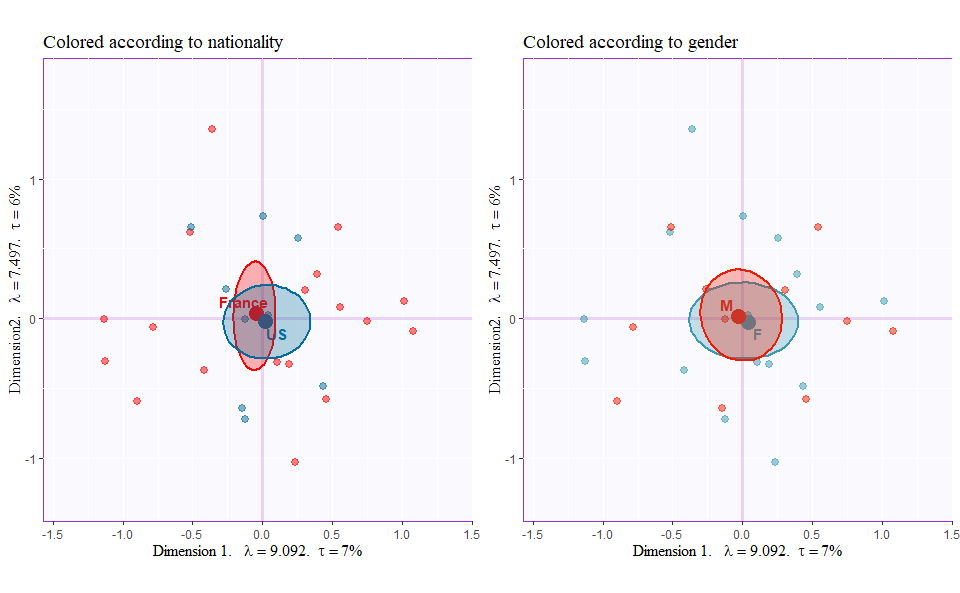
\includegraphics{./supmatsimgs/qrvplot.png}
  \label{fig:qrvplot}
  \caption*{\footnotesize \textit{Note.} Axis labels indicate dimension, eigenvalue, and explained variance for that dimension.}
\end{figure}

\begin{figure}   
  \centering  
  \caption{Hierarchical cluster analysis for the row factor scores of the CA for Experiment 1.}
    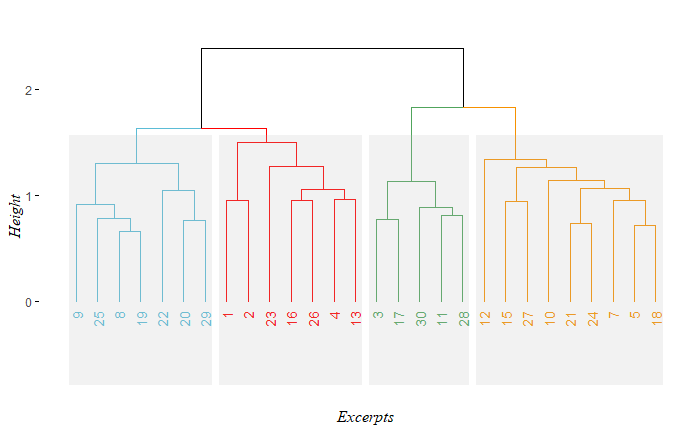
\includegraphics{./supmatsimgs/qhca1.png}
  \label{fig:qhca1}
\end{figure}

\begin{figure}   
  \centering  
  \caption{Hierarchical cluster analysis for the row factor scores of the CA for Experiment 1 including Excerpts 6 and 14.}
    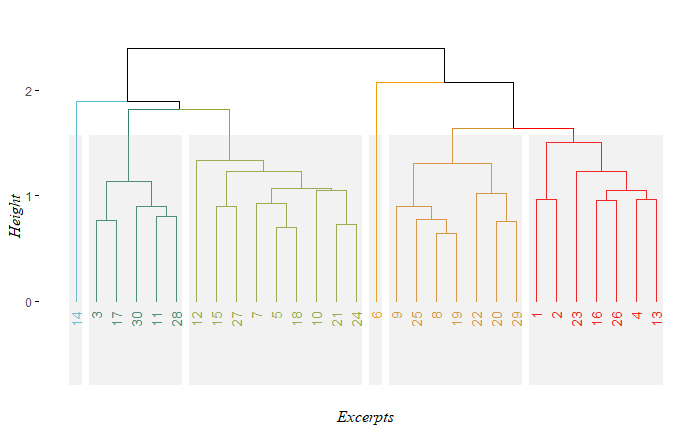
\includegraphics{./supmatsimgs/qhca2.png}
  \label{fig:qhca2}

\end{figure}

\begin{figure}   
  \centering  
  \caption{CA: Row factor scores for preliminary analysis of the qualities survey, featuring Dimensions 1 and 2, with tolerance intervals around the clusters identified by the HCA.}
    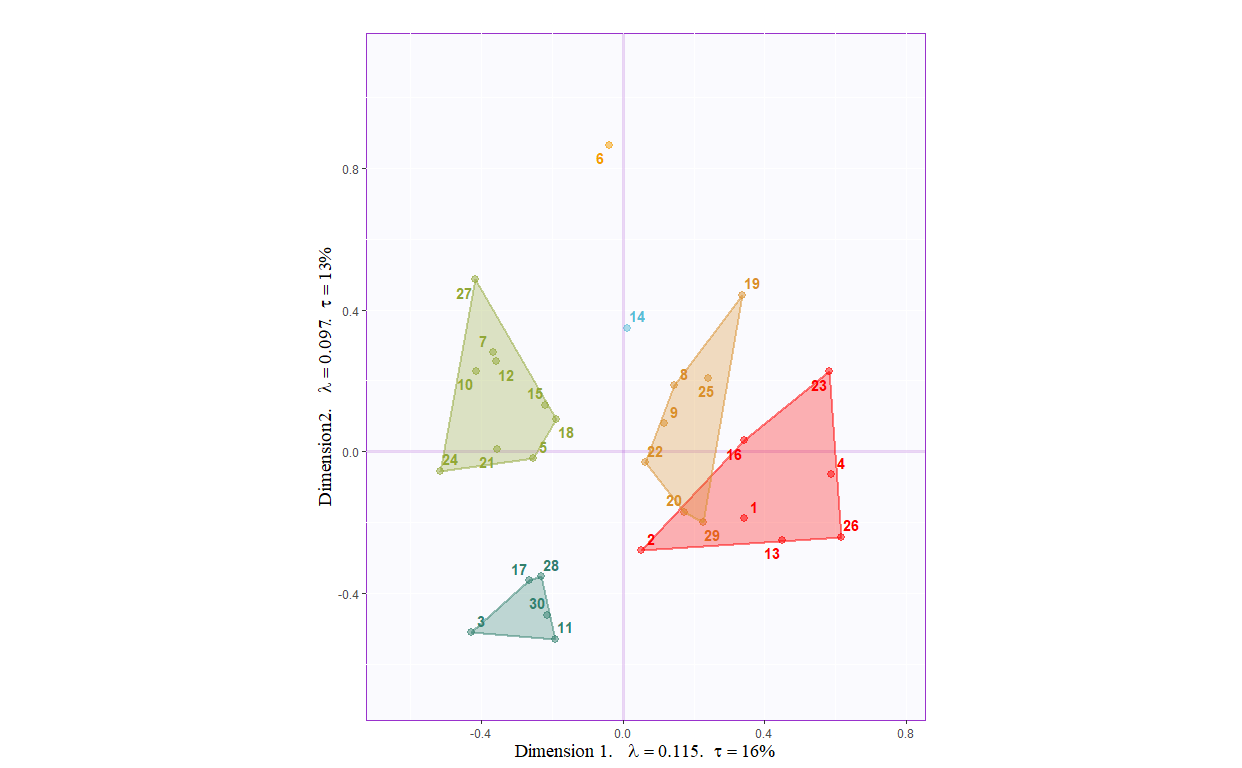
\includegraphics{./supmatsimgs/qfactormap12.png}
  \label{fig:qimap12}
  \caption*{\footnotesize \textit{Note.} Axis labels indicate dimension, eigenvalue, and explained variance for that dimension.}
\end{figure}

\begin{figure}   
  \centering  
  \caption{CA: Row factor scores for the preliminary analysis of the qualities survey, featuring Dimensions 2 and 3, with tolerance intervals around the clusters identified by the HCA.}
    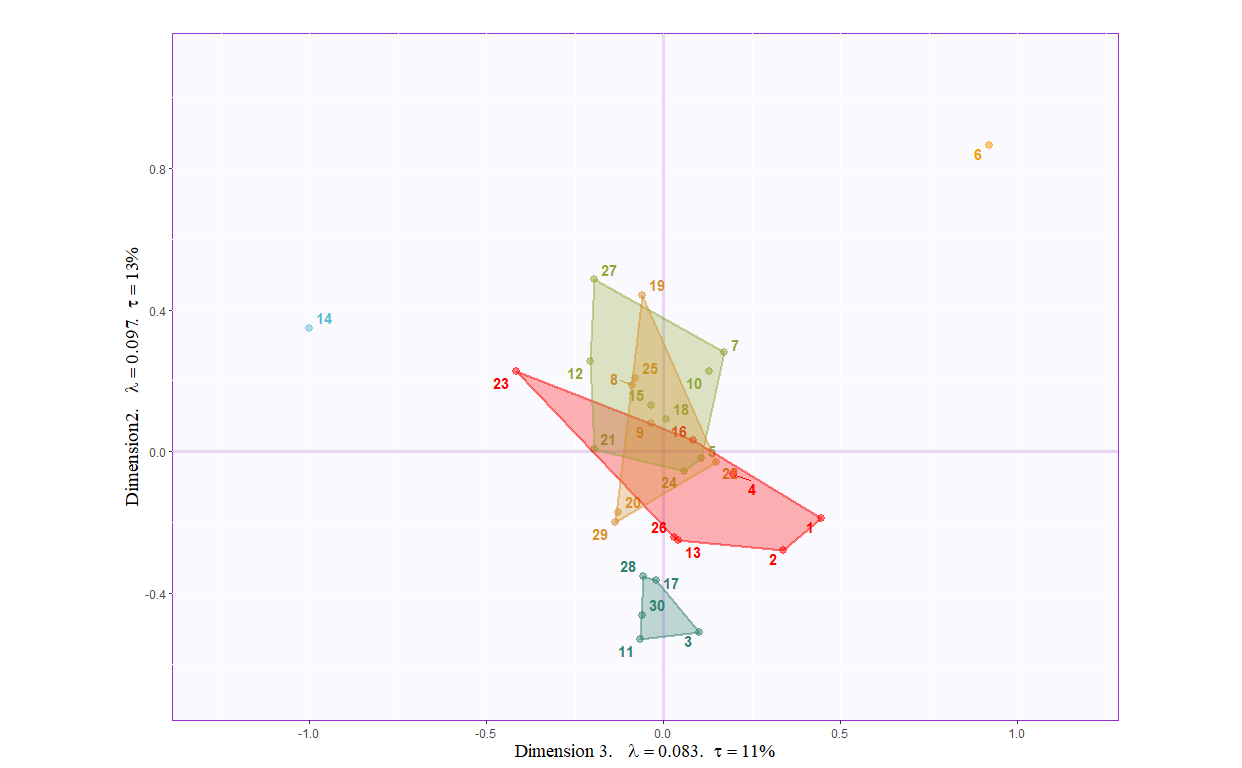
\includegraphics{./supmatsimgs/qfactormap23.png}
  \label{fig:qimap23}
  \caption*{\footnotesize \textit{Note.} Axis labels indicate dimension, eigenvalue, and explained variance for that dimension.}
\end{figure}

\begin{figure}   
  \centering  
  \caption{CA: Column factor scores for the analysis of the qualities survey, points are levels of each variable, colored by variable.}
    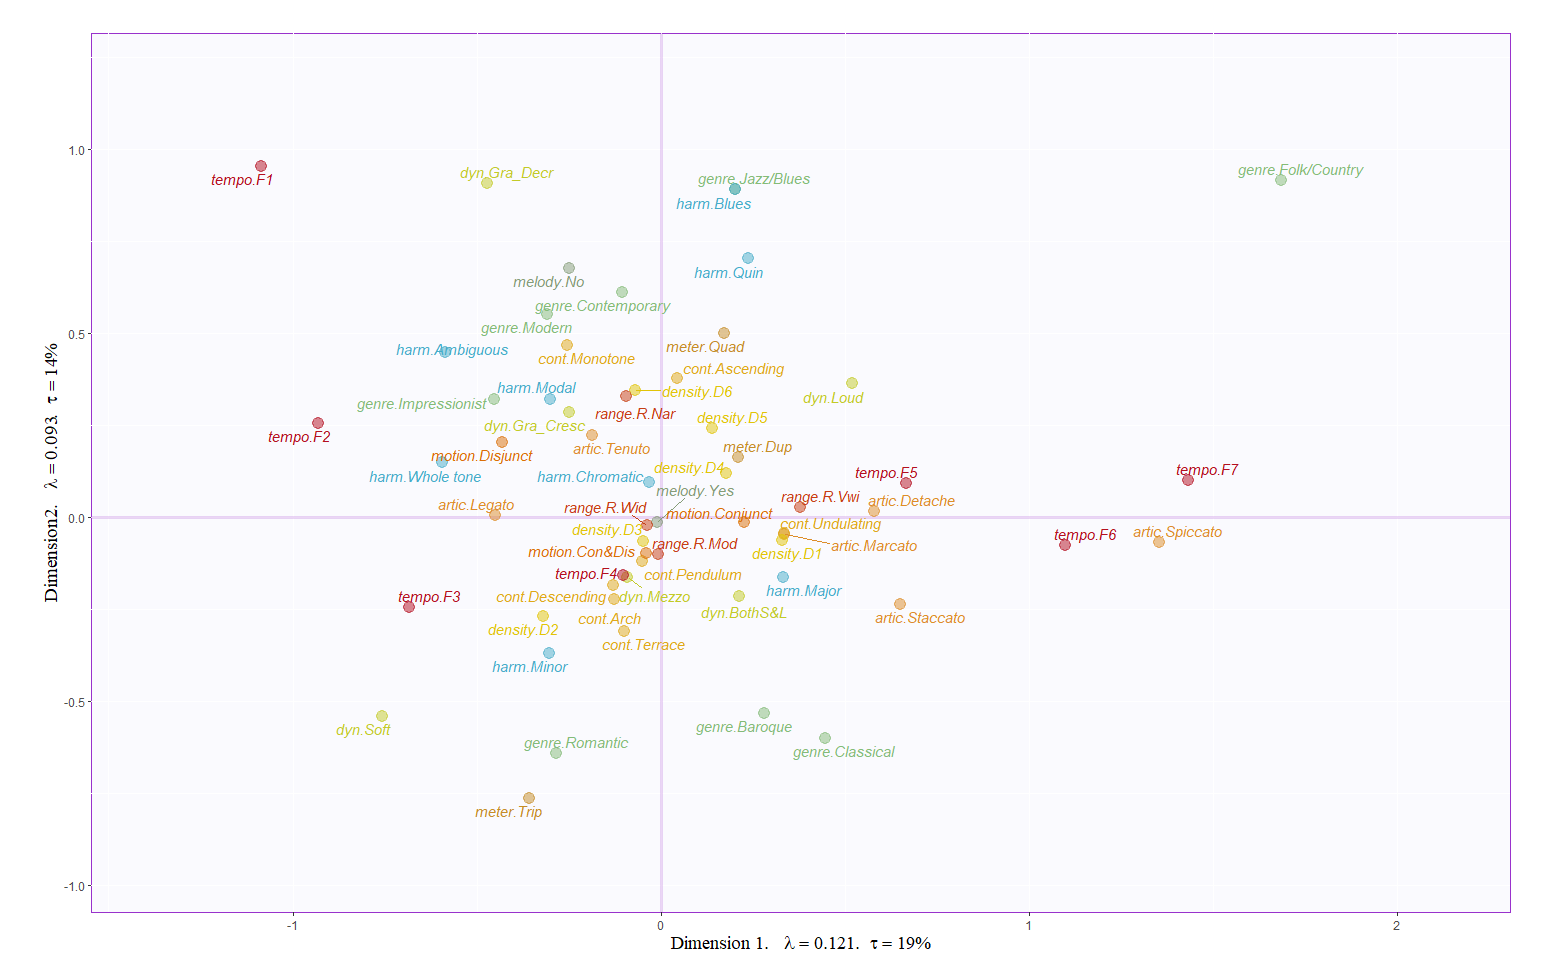
\includegraphics{./supmatsimgs/qfactormapsjall.png}
  \label{fig:qjmapsall}
  \caption*{\footnotesize \textit{Note.} Axis labels indicate dimension, eigenvalue, and explained variance for that dimension.}
\end{figure}

```\{= latex\}

\begin{figure}
\caption{Separate plots for each of the qualities evaluated in the musical qualities survey}
\centering
\begin{subfigure}[b]{.45\linewidth}
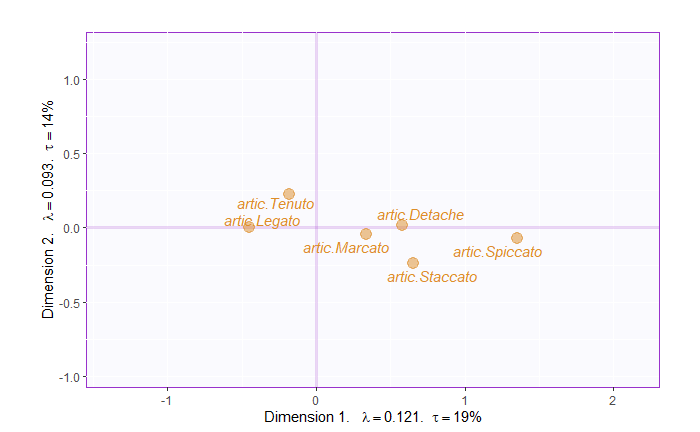
\includegraphics[width=\linewidth]{./supmatsimgs/qjartic.png}
\caption{Articulations}\label{fig:artic}
\end{subfigure}
\begin{subfigure}[b]{.45\linewidth}
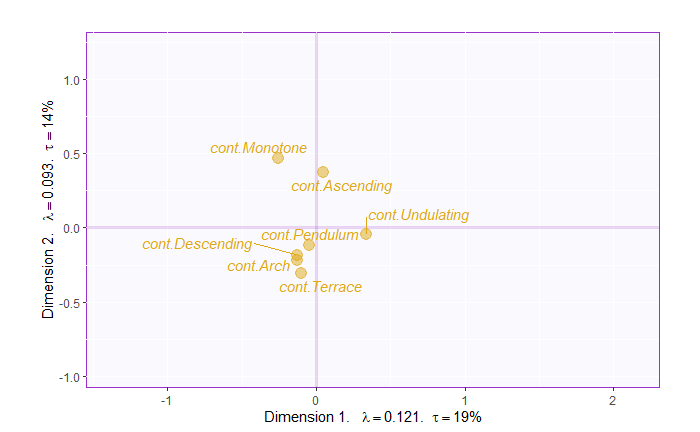
\includegraphics[width=\linewidth]{./supmatsimgs/qjcontour.png}
\caption{Contour}\label{fig:contour}
\end{subfigure}

\begin{subfigure}[b]{.45\linewidth}
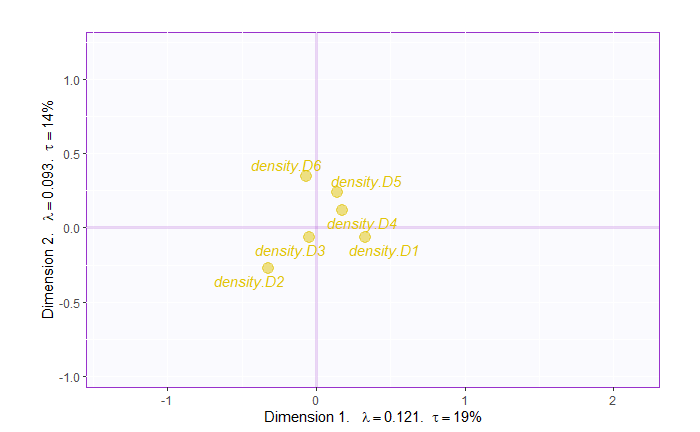
\includegraphics[width=\linewidth]{./supmatsimgs/qjdensity.png}
\caption{Density}\label{fig:density}
\end{subfigure}
\begin{subfigure}[b]{.45\linewidth}
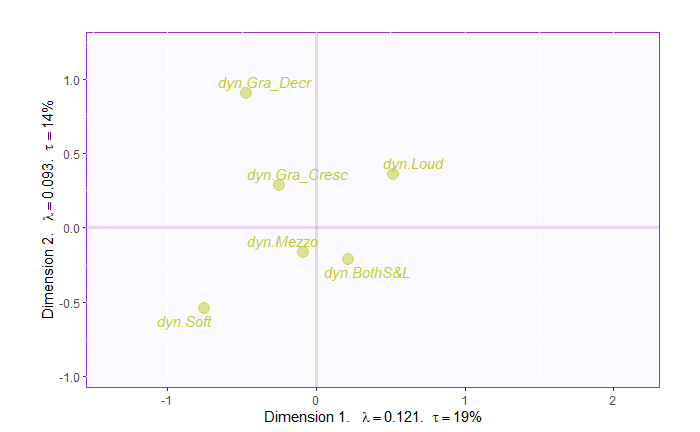
\includegraphics[width=\linewidth]{./supmatsimgs/qjdynamics.png}
\caption{Dynamics}\label{fig:dynamics}
\end{subfigure}

\begin{subfigure}[b]{.45\linewidth}
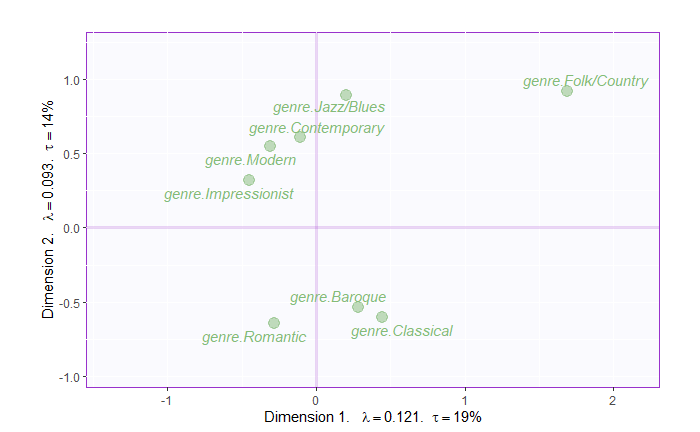
\includegraphics[width=\linewidth]{./supmatsimgs/qjgenre.png}
\caption{Genre}\label{fig:genre}
\end{subfigure}
\begin{subfigure}[b]{.45\linewidth}
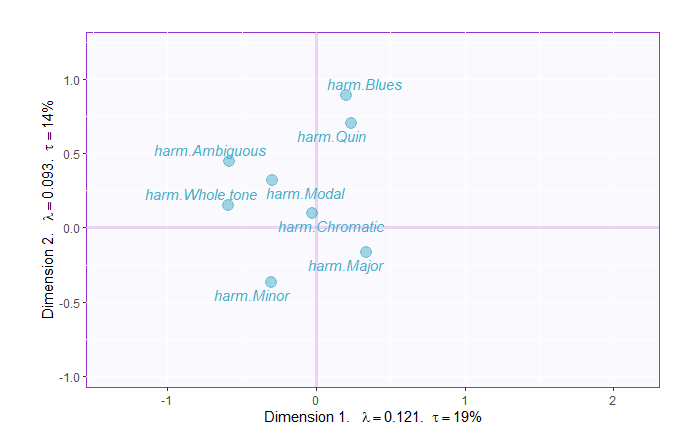
\includegraphics[width=\linewidth]{./supmatsimgs/qjharmony.png}
\caption{Harmony}\label{fig:harmony}
\end{subfigure}

\begin{subfigure}[b]{.45\linewidth}
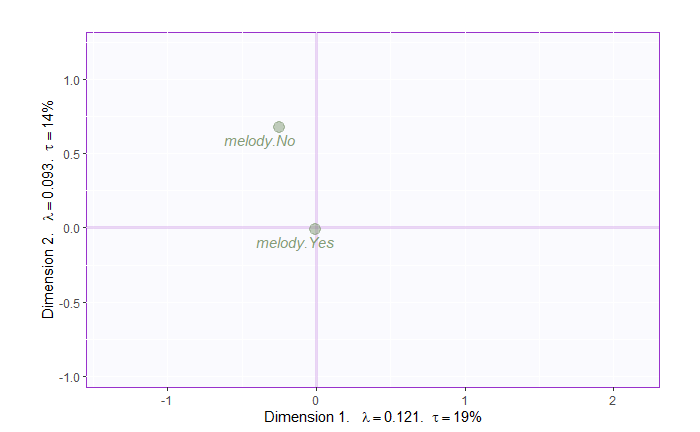
\includegraphics[width=\linewidth]{./supmatsimgs/qjmelody.png}
\caption{Melody}\label{fig:melody}
\end{subfigure}
\begin{subfigure}[b]{.45\linewidth}
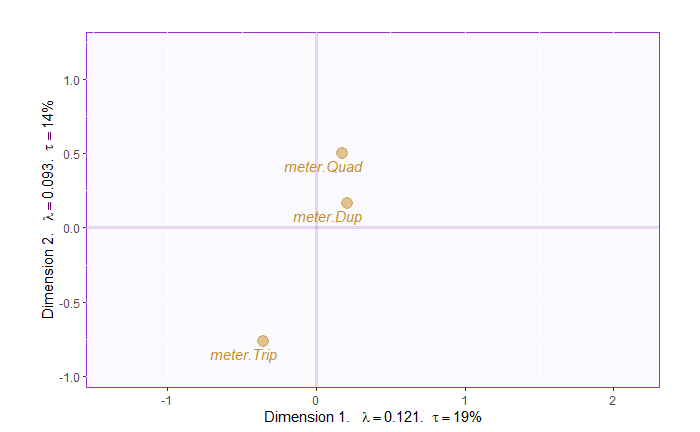
\includegraphics[width=\linewidth]{./supmatsimgs/qjmeter.png}
\caption{Meter}\label{fig:meter}
\end{subfigure}
\end{figure}

\begin{figure}[ht]\ContinuedFloat
\centering
\begin{subfigure}[b]{.45\linewidth}
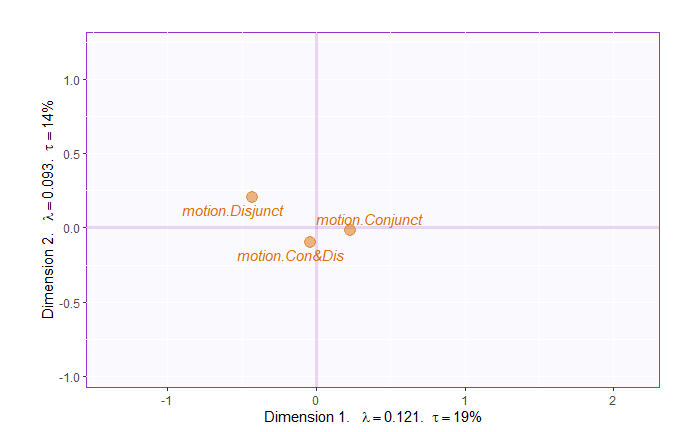
\includegraphics[width=\linewidth]{./supmatsimgs/qjmotion.png}
\caption{Motion}\label{fig:motion}
\end{subfigure}
\begin{subfigure}[b]{.45\linewidth}
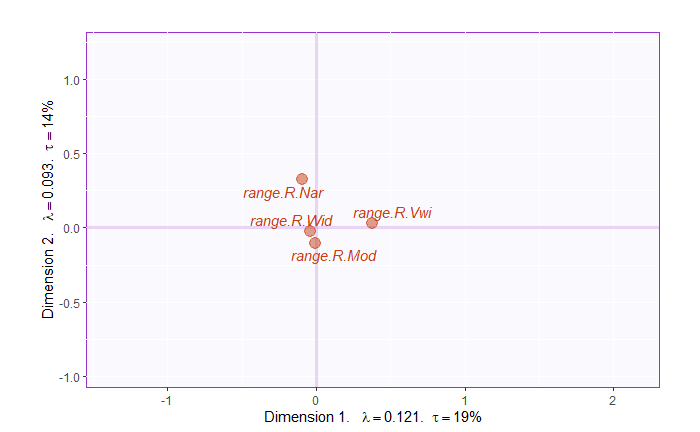
\includegraphics[width=\linewidth]{./supmatsimgs/qjrange.png}
\caption{Range}\label{fig:range}
\end{subfigure}

\begin{subfigure}[b]{.45\linewidth}
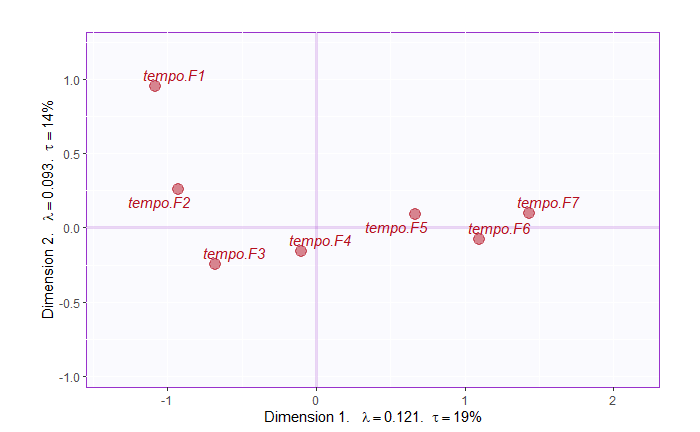
\includegraphics[width=\linewidth]{./supmatsimgs/qjtempo.png}
\caption{Tempo}\label{fig:tempo}
\end{subfigure}

\label{fig:qualities}
\end{figure}

\begin{sidewaysfigure}  
  \centering  
  \caption{CA: All Row and column contributions for the first two dimensions of the qualities survey.}
    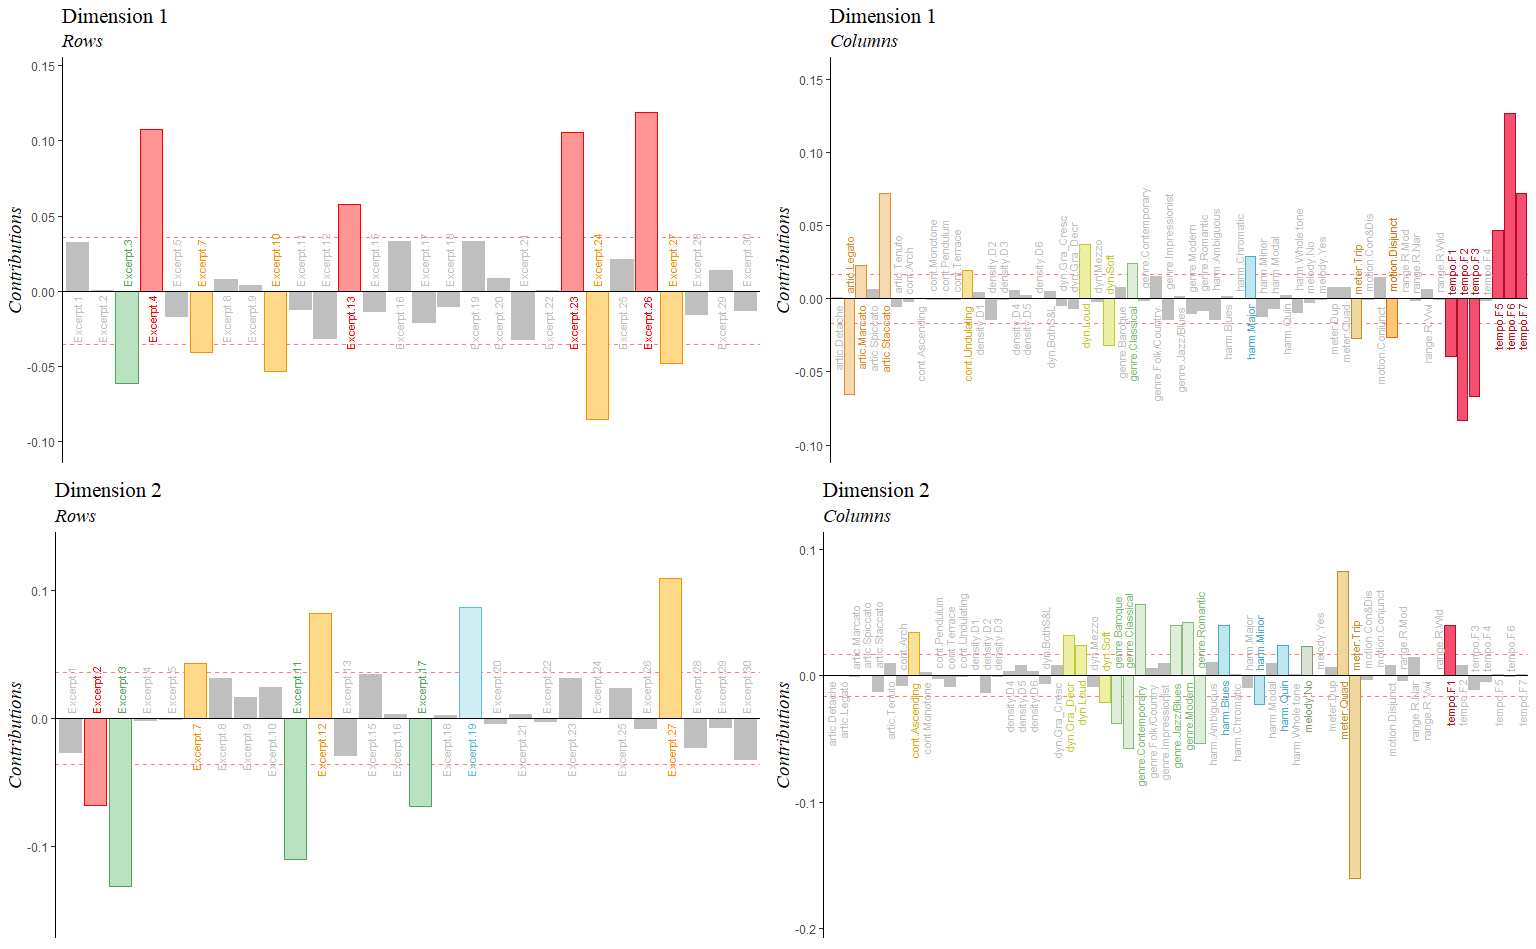
\includegraphics{./supmatsimgs/qconts.png}
  \label{fig:qconts}
\end{sidewaysfigure}

\begin{verbatim}
# Supplementary Materials: Experiment 2


\begin{table}[H]

\begin{center}
\begin{threeparttable}

\caption{\label{tab:adjtable}CATA Adjectives}

\begin{tabular}{ll}
\toprule
English & \multicolumn{1}{c}{French}\\
\midrule
Slow & Lent\\
Fast & Rapide\\
Dense & Bavard\\
Sparse & Epure\\
Complex & Complexe\\
Transparent & Transparent\\
Light & Clair\\
Dark & Sombre\\
Bright & Brillant\\
Dull & Terne\\
Soft & Doux\\
Strong & Fort\\
Mysterious & Mysterieux\\
Melancholy & Melancolique\\
Incisive & Incisif\\
Round & Tendre\\
Aggressive & Agressif\\
Weak & Faible\\
Strong & Puissant\\
Warm & Chaleureux\\
Solemn & Solennel\\
Valiant & Vaillant\\
Sad & Triste\\
Happy & Joyeux\\
Dancing & Dansant\\
Disturbing & Inquietant\\
Exotic & Exotique\\
Colorful & Colore\\
Varied & Changeant\\
Monotonous & Monotone\\
Long & Long\\
Short & Court\\
Surprising & Surprenant\\
\bottomrule
\end{tabular}

\end{threeparttable}
\end{center}

\end{table}



```{=latex}

\begin{figure}   
  \centering  
  \caption{Hierarchical cluster analysis for the row factor scores of the CA for Experiment 2.}
    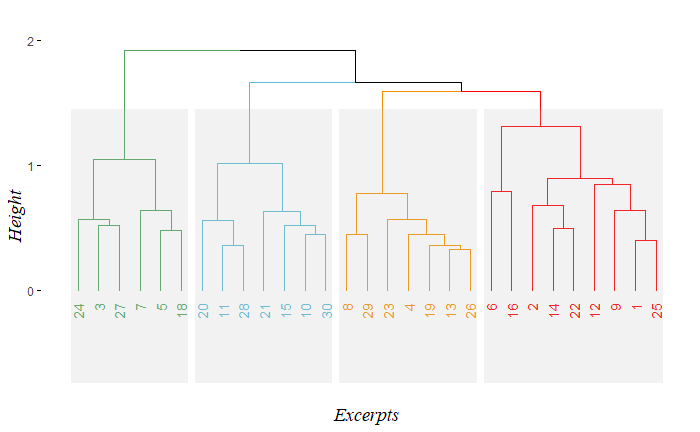
\includegraphics{./supmatsimgs/ahca1.png}
  \label{fig:ahca1}
\end{figure}
\end{verbatim}

\begin{figure}   
  \centering  
  \caption{Hierarchical cluster analysis for the column factor scores of the CA for Experiment 2.}
    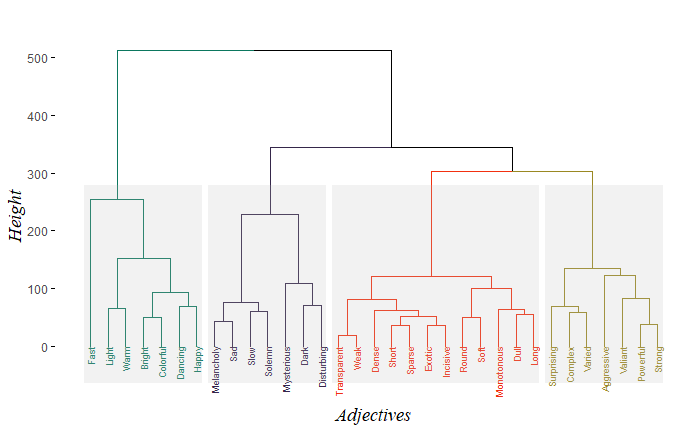
\includegraphics{./supmatsimgs/ahca2.png}
  \label{fig:ahca2}
\end{figure}

\begin{figure}   
  \centering  
  \caption{CA: Row and column factor scores for the first two dimensions of the CA for Experiment 2.}
    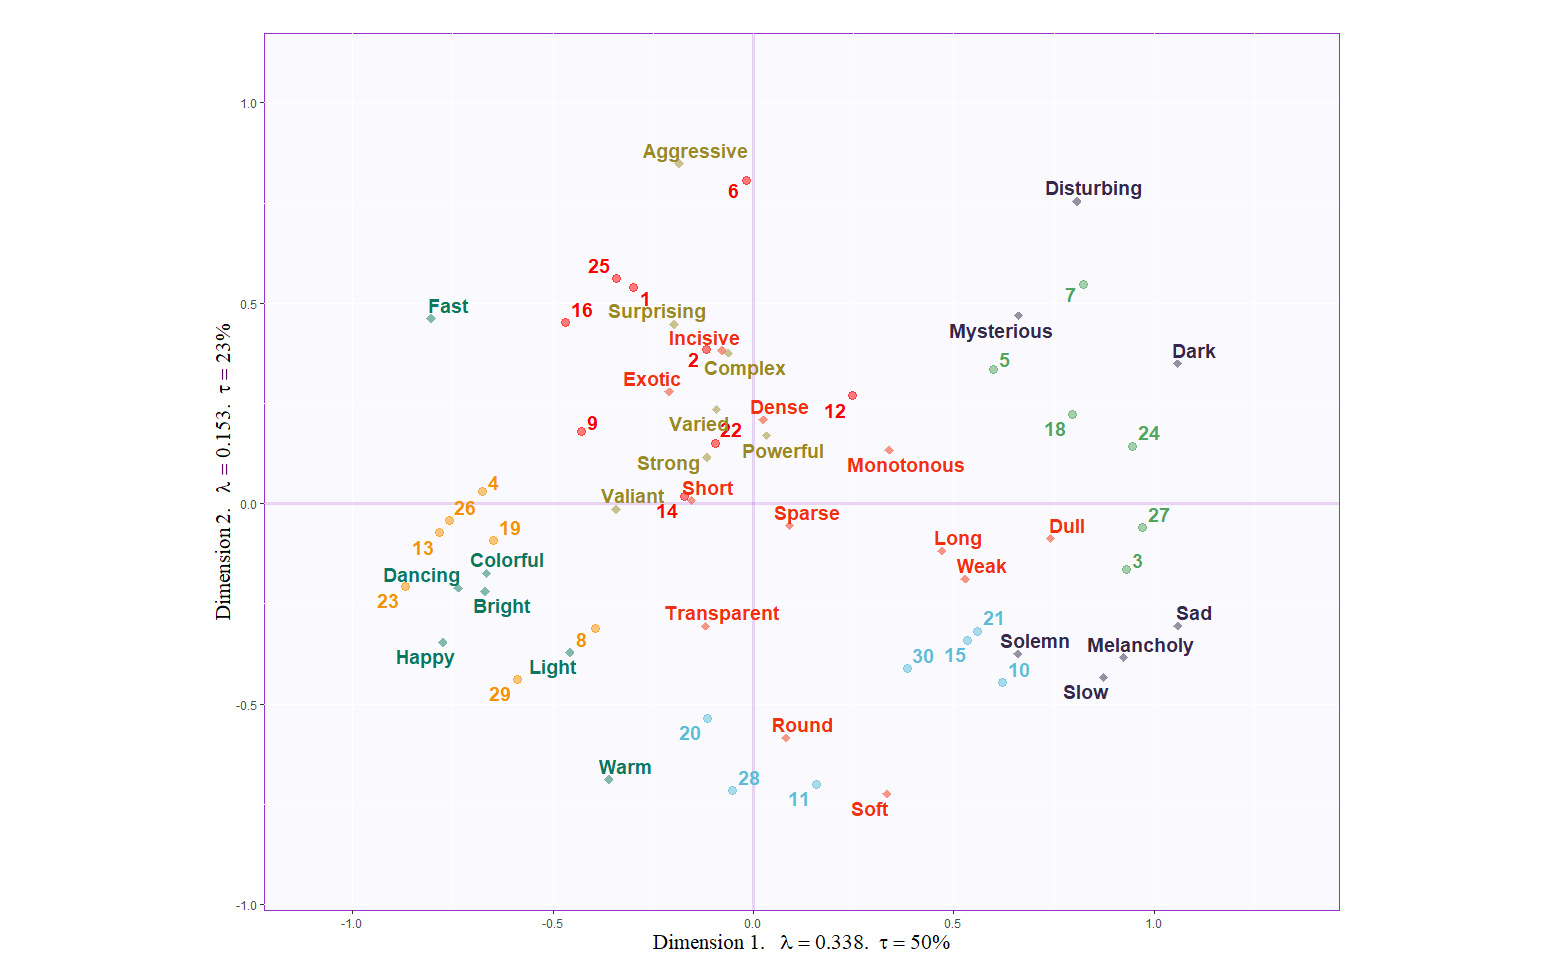
\includegraphics{./supmatsimgs/asym.png}
  \label{fig:asym}
  \caption*{\footnotesize \textit{Note.} Axis labels indicate dimension, eigenvalue, and explained variance for that dimension.}
\end{figure}

\begin{figure}   
  \centering  
  \caption{CA: Row and column factor scores for the first two dimensions of the CA for Experiment 2.}
    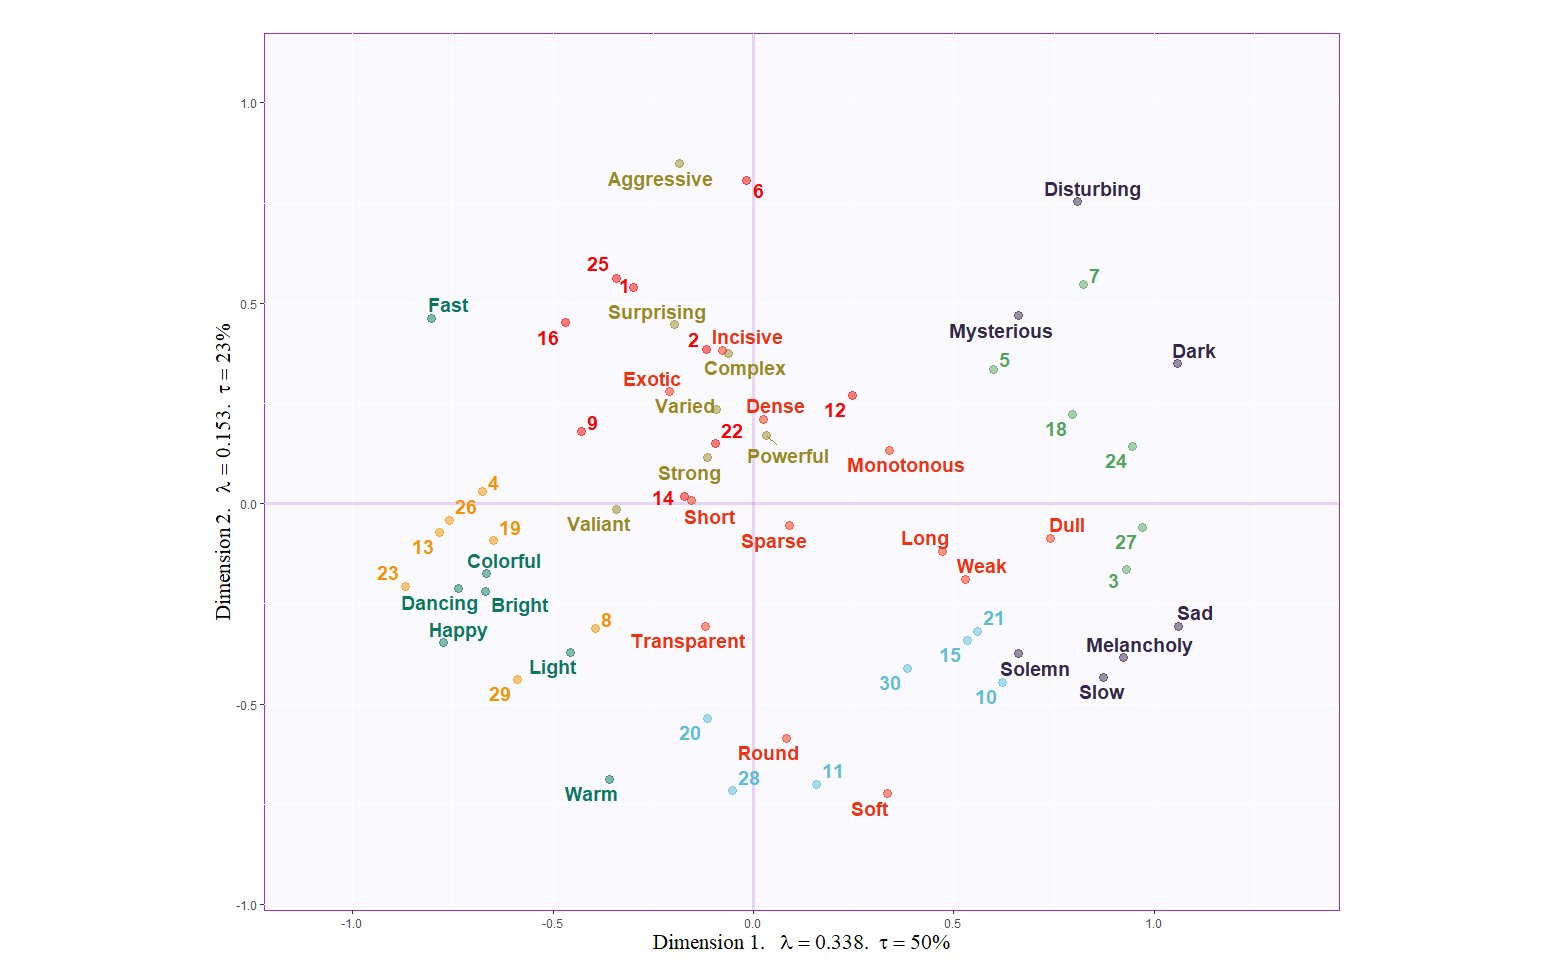
\includegraphics{./supmatsimgs/asymrepel.png}
  \label{fig:asymrepel}
  \caption*{\footnotesize \textit{Note.} Axis labels indicate dimension, eigenvalue, and explained variance for that dimension.}
\end{figure}

\begin{figure}   
  \centering  
  \caption{CA: All Row and column contributions for the first two dimensions of the adjectives survey.}
    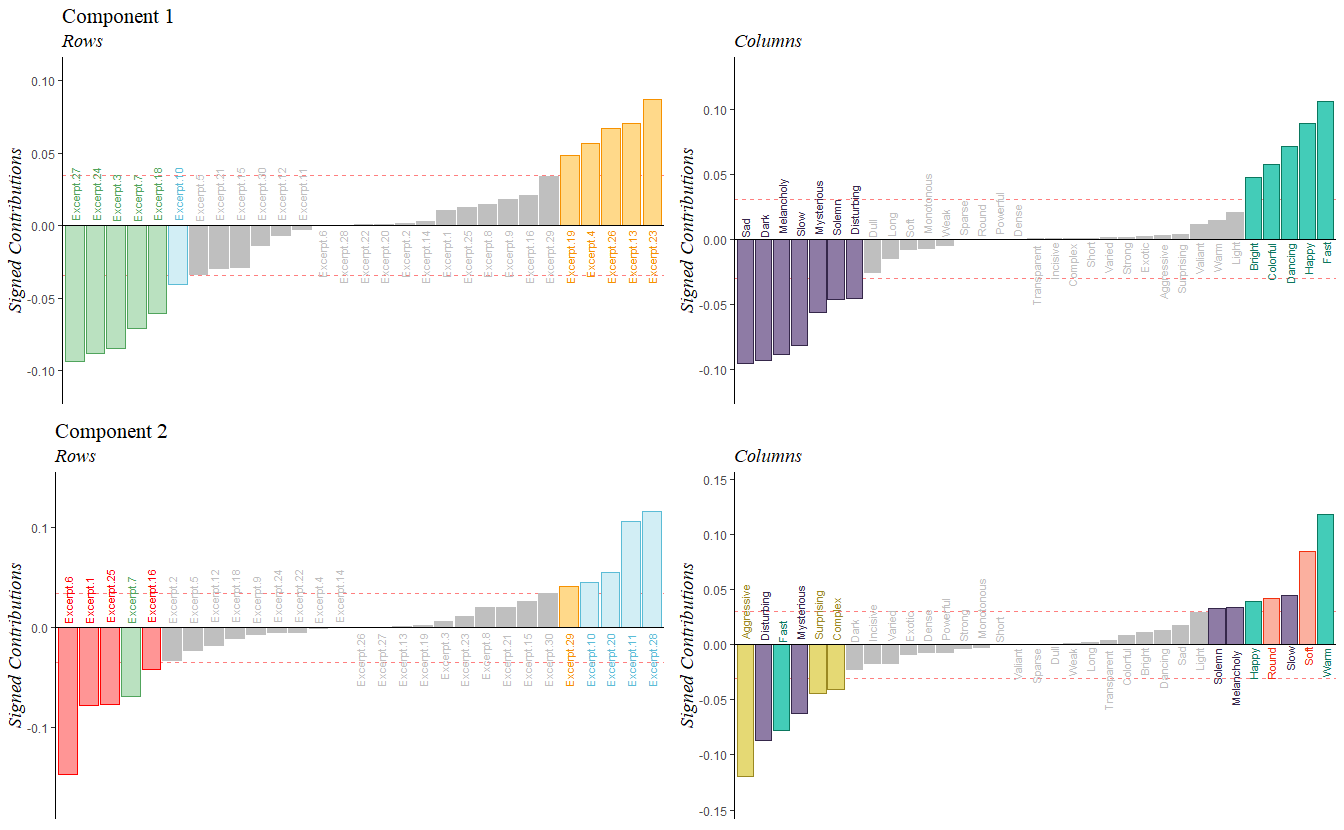
\includegraphics{./supmatsimgs/acontsordered.png}
  \label{fig:aconts}
\end{figure}

\begin{figure}   
  \centering  
  \caption{PLSC: Correlation matrix for the columns of the surveys from Experiments 1 and 2. Correlation values between variables are indicated by color and opacity. Dark blue is a strong positive correlation and dark red is a strong negative correlation, pale or white squares indicate little to no correlation.}
    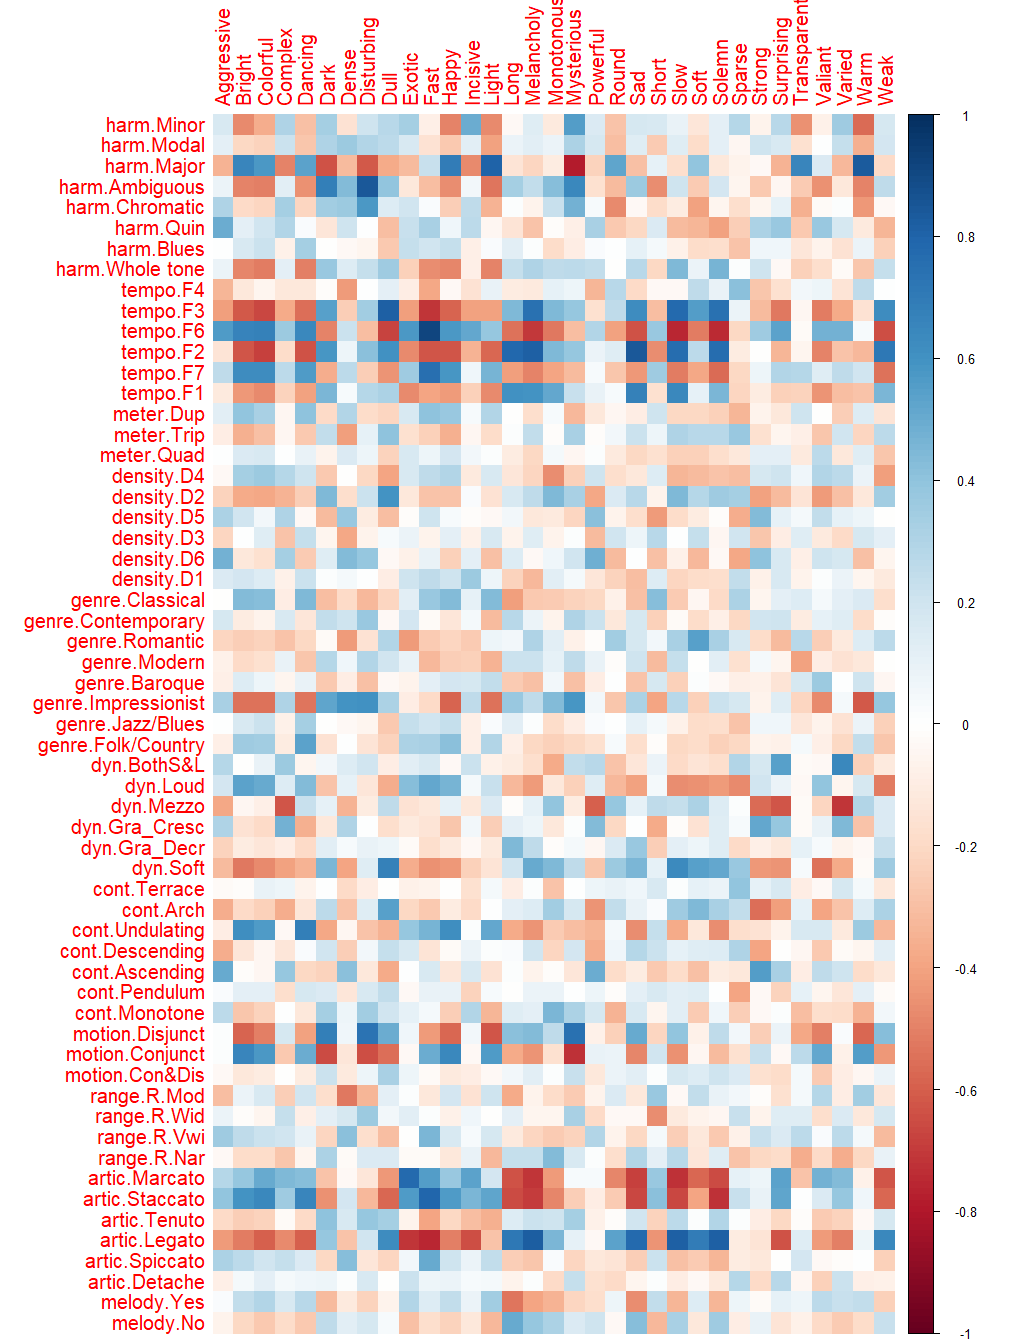
\includegraphics{./supmatsimgs/pcorrplot.png}
  \label{fig:pcorr}
\end{figure}

\begin{figure}   
  \centering  
  \caption{PLSC: loadings barplots for the columns of the surveys from Experiments 1 and 2. The loading on a dimension for a variable is the square of its contribution to that dimension.}
    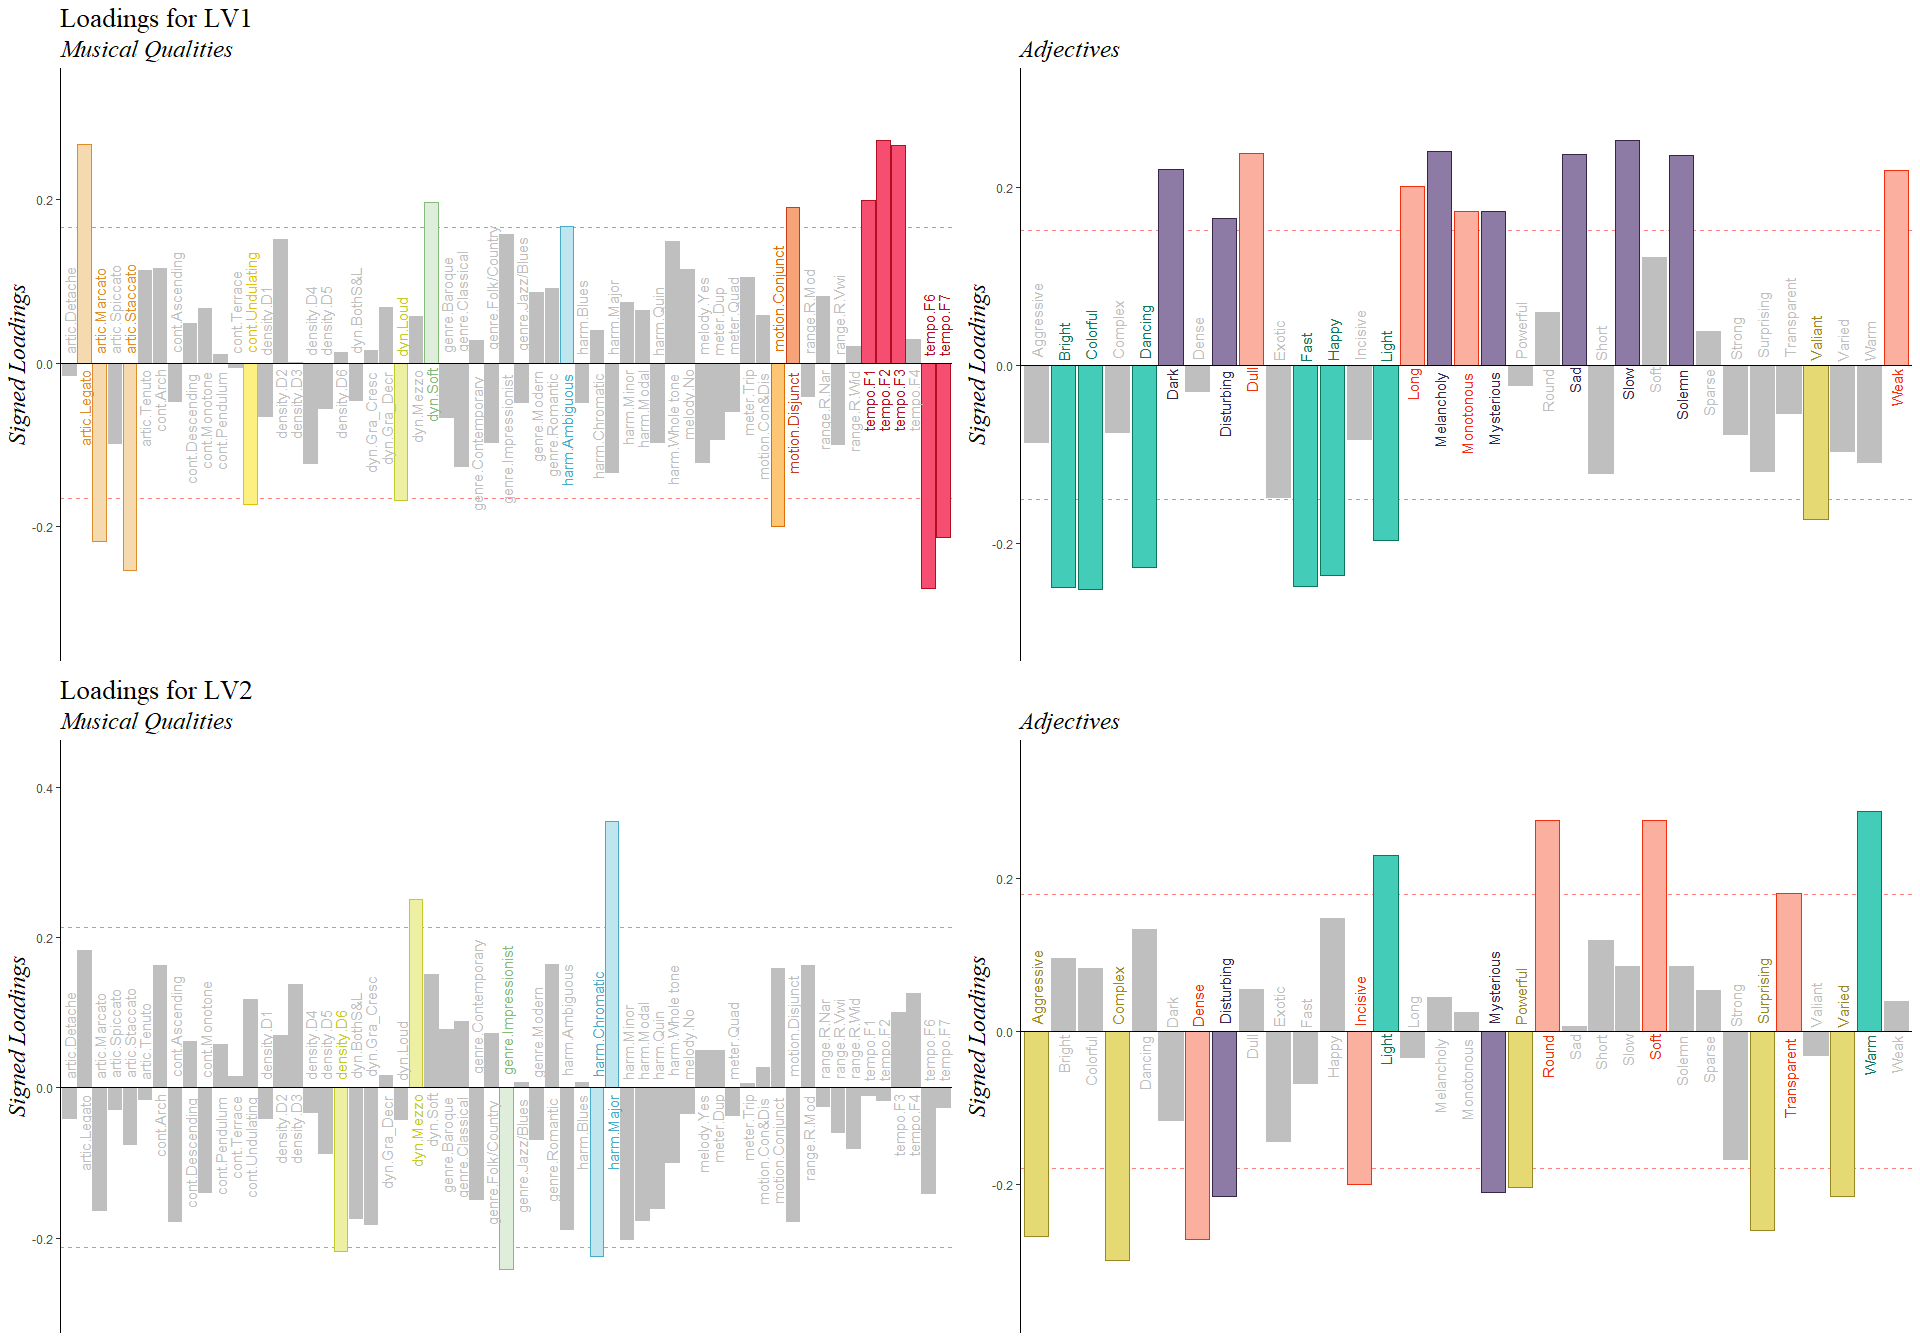
\includegraphics{./supmatsimgs/ploads.png}
  \label{fig:ploads}
\end{figure}

\end{document}
